\documentclass[thesis.tex]{subfiles}

\pagebreak
\appendix
\chapter{Application examples}
This section showcases some examples of the BK.Synapse web application.

\begin{figure}[htp]
	\centering
	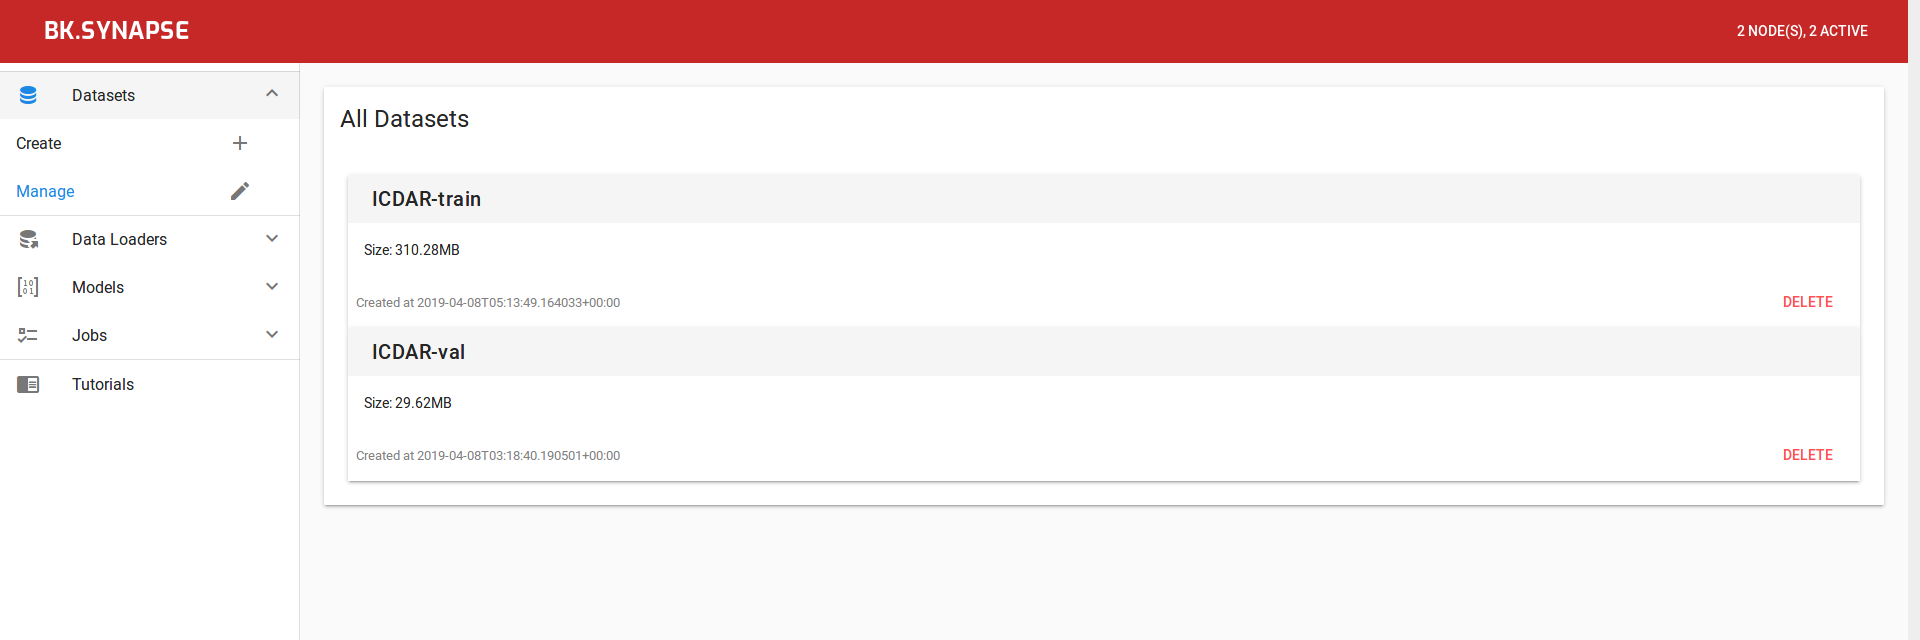
\includegraphics[width=0.95\textwidth,frame]{bks_example_2.png}
	\caption{Managing datasets}
	\label{fig:example-2}
\end{figure}
\begin{figure}[htp]
	\centering
	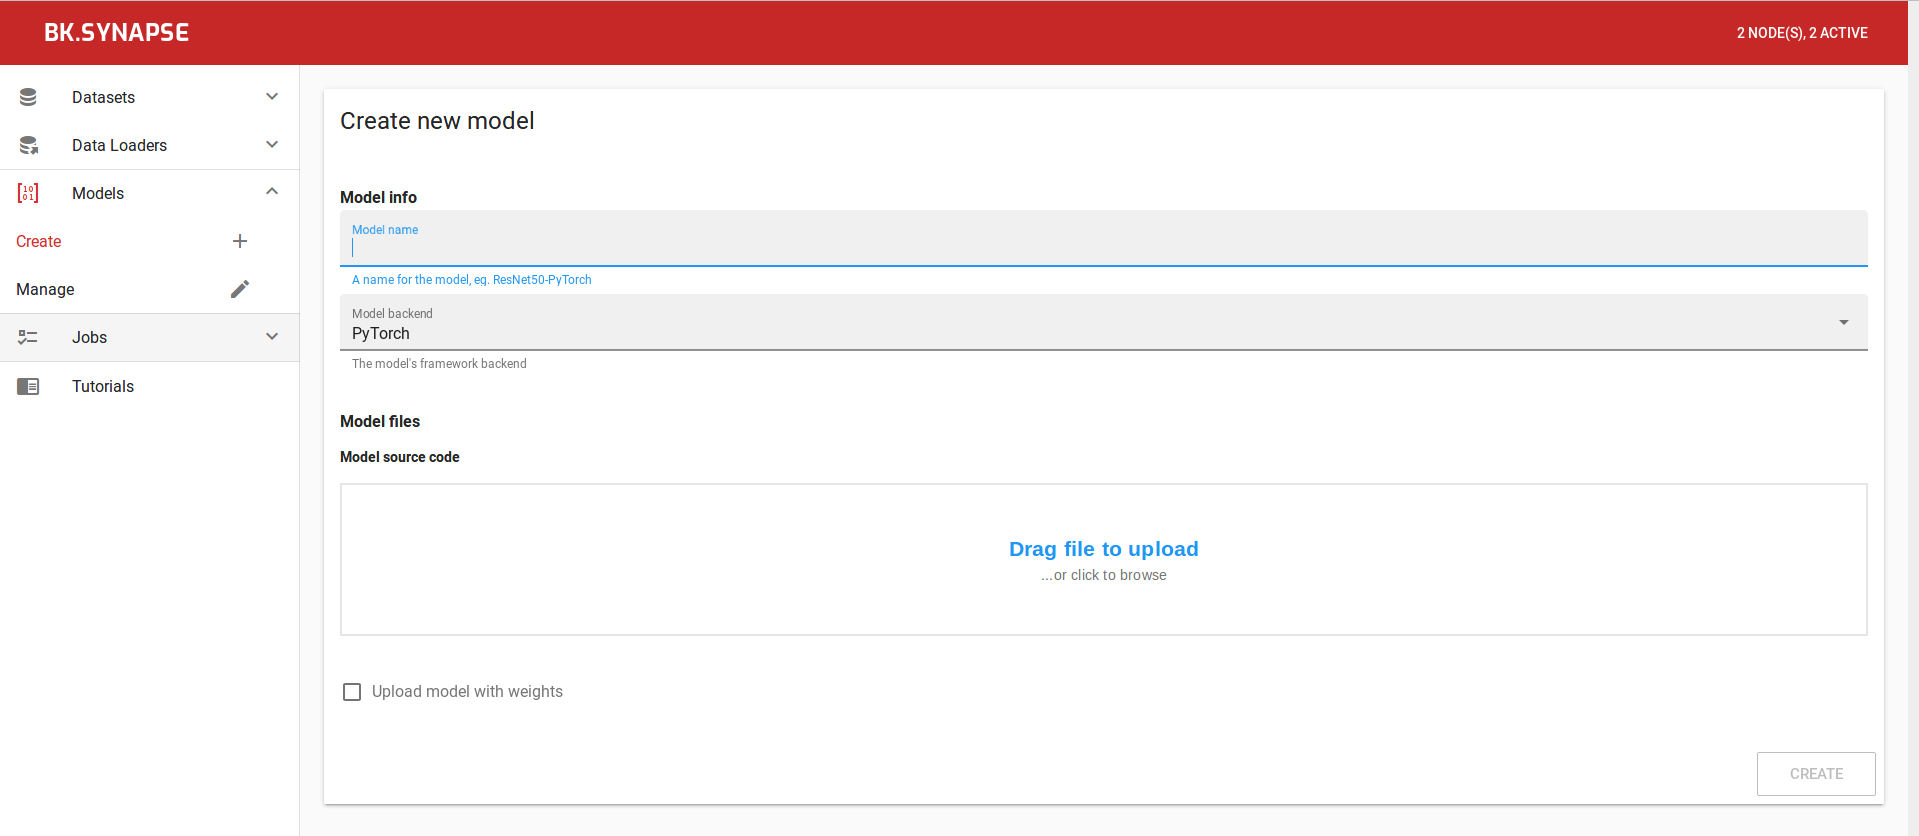
\includegraphics[width=0.95\textwidth,frame]{bks_example_3.png}
	\caption{Creating new models}
	\label{fig:example-3}
\end{figure}
\begin{figure}[htp]
	\centering
	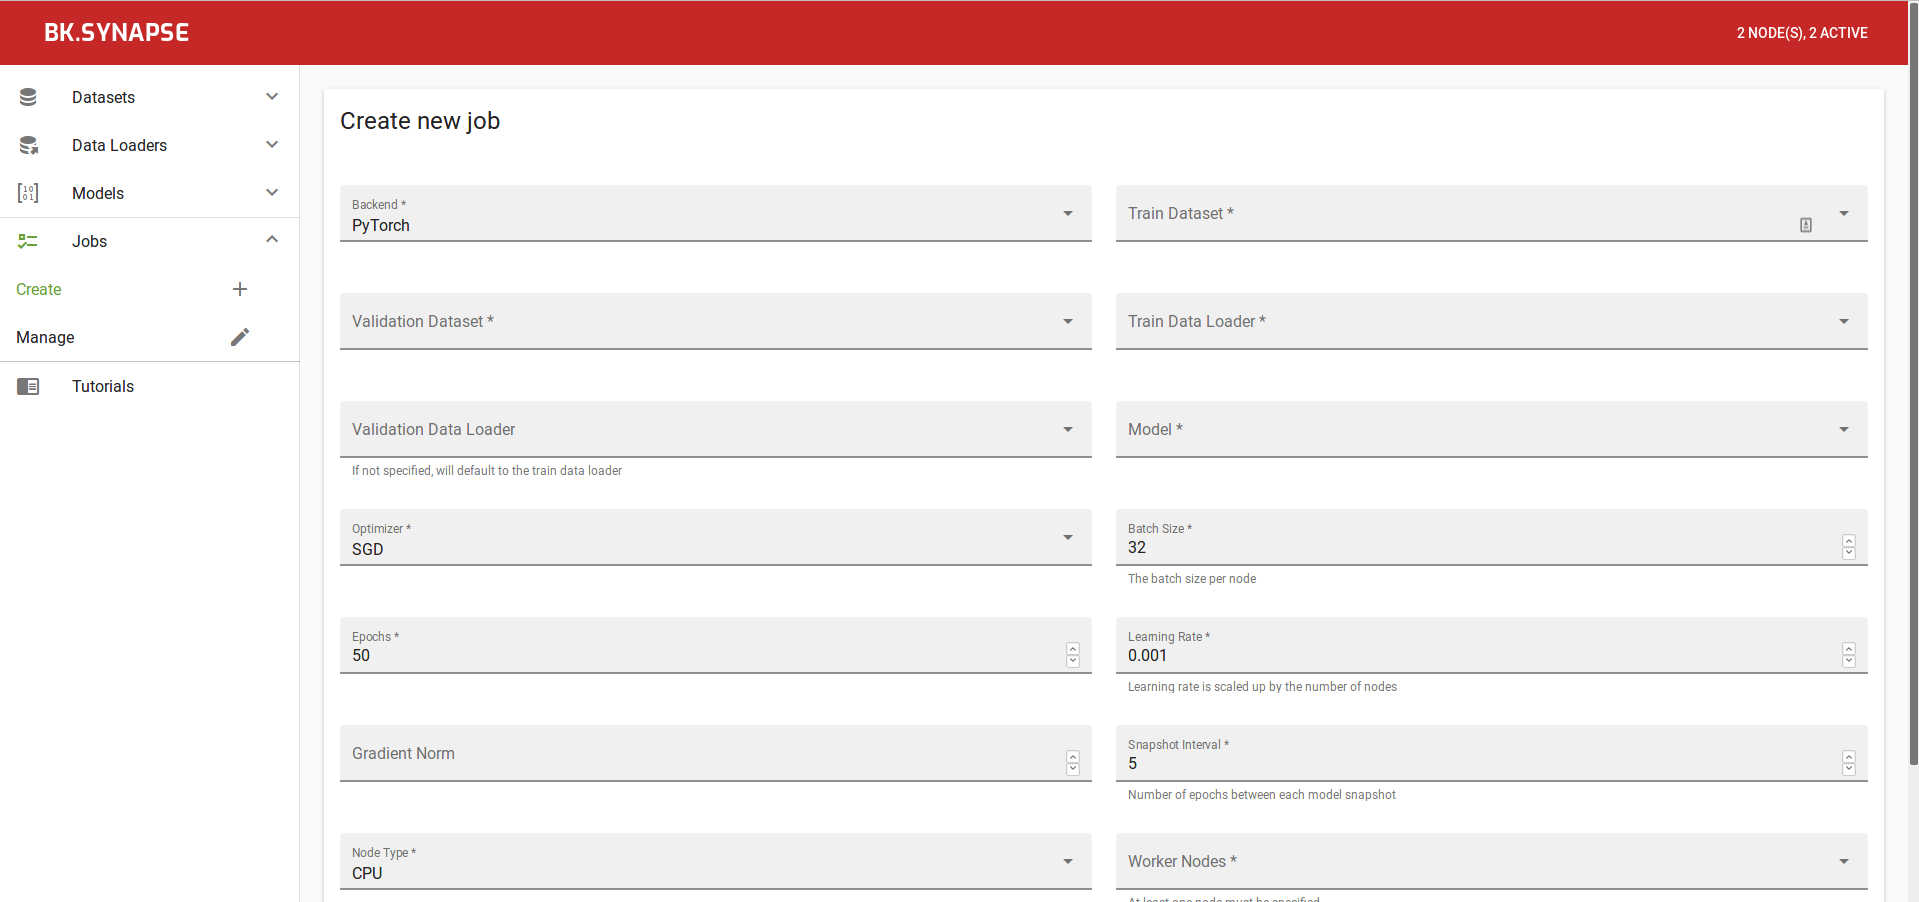
\includegraphics[width=0.95\textwidth,frame]{bks_example_4.png}
	\caption{Job creation form}
	\label{fig:example-4}
\end{figure}
\begin{figure}[htp]
	\centering
	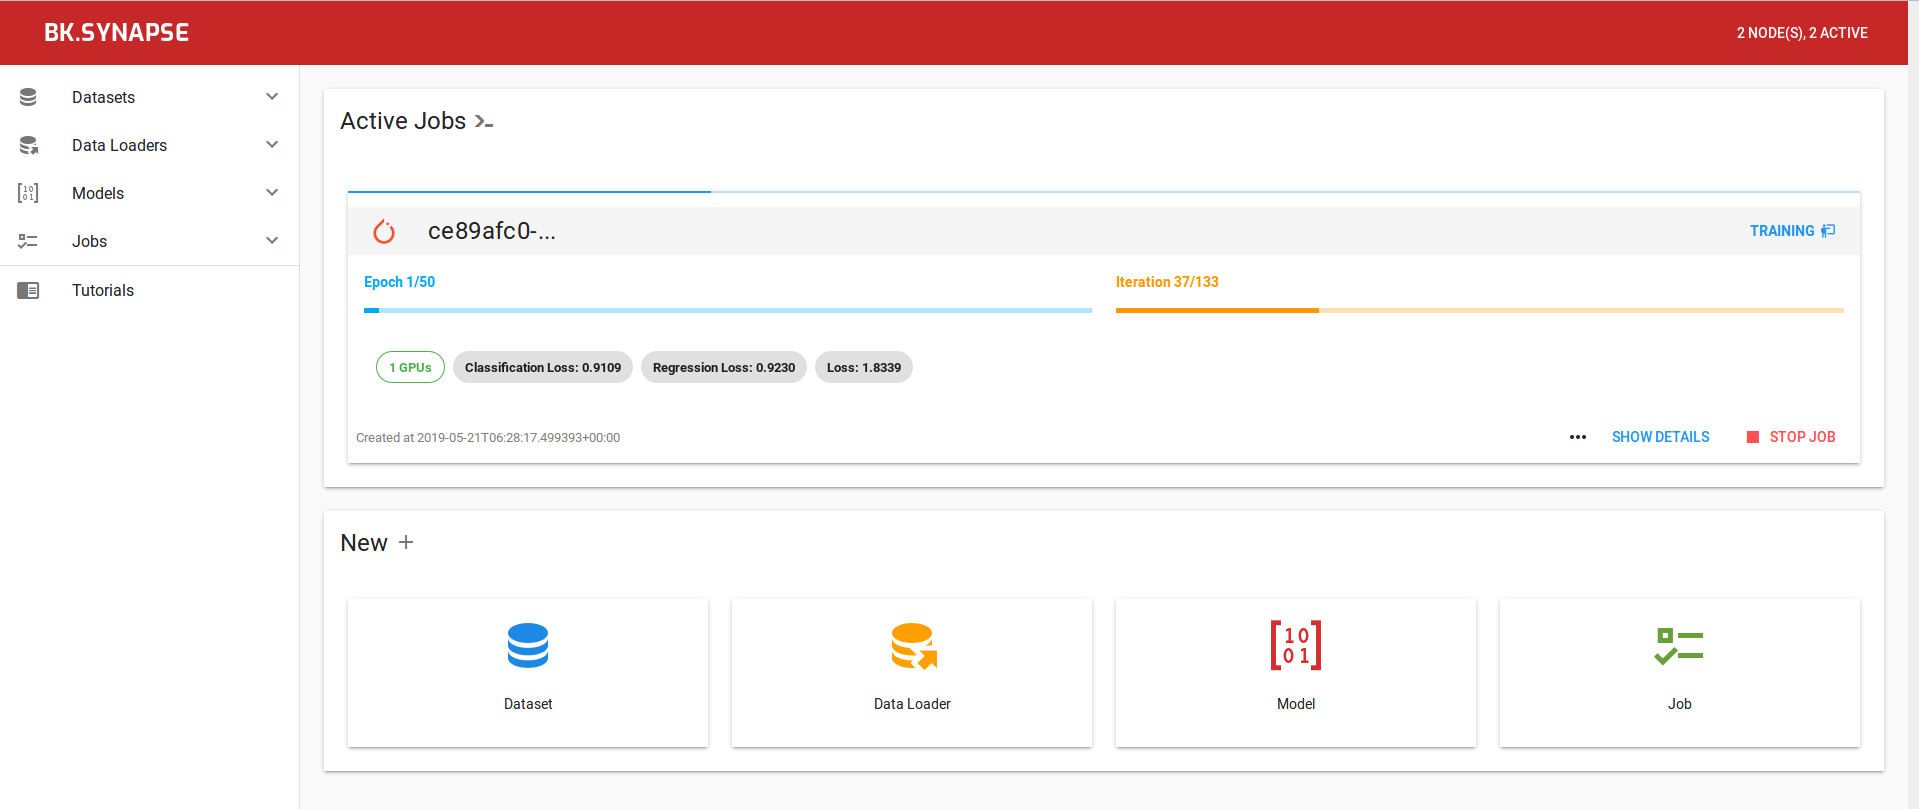
\includegraphics[width=0.95\textwidth,frame]{bks_example_5.png}
	\caption{Main UI showing active jobs}
	\label{fig:example-5}
\end{figure}
\begin{figure}[htp]
	\centering
	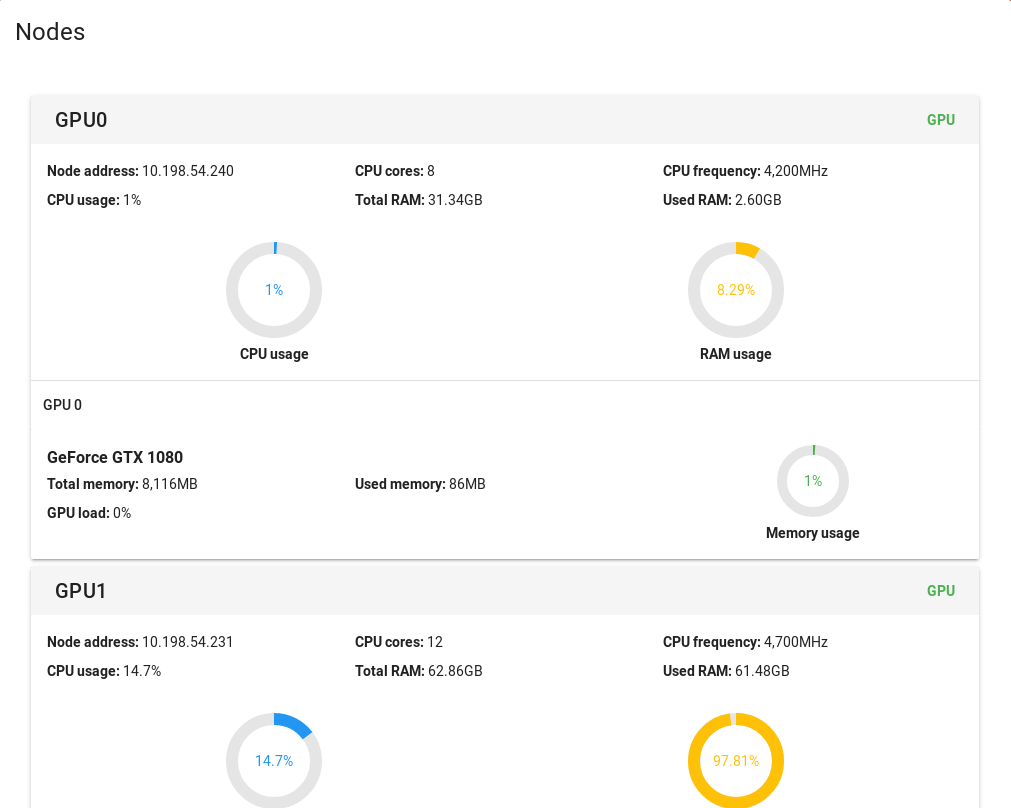
\includegraphics[width=0.95\textwidth,frame]{bks_example_6.png}
	\caption{Node hardware statistics}
	\label{fig:example-6}
\end{figure}
\begin{figure}[htp]
	\centering
	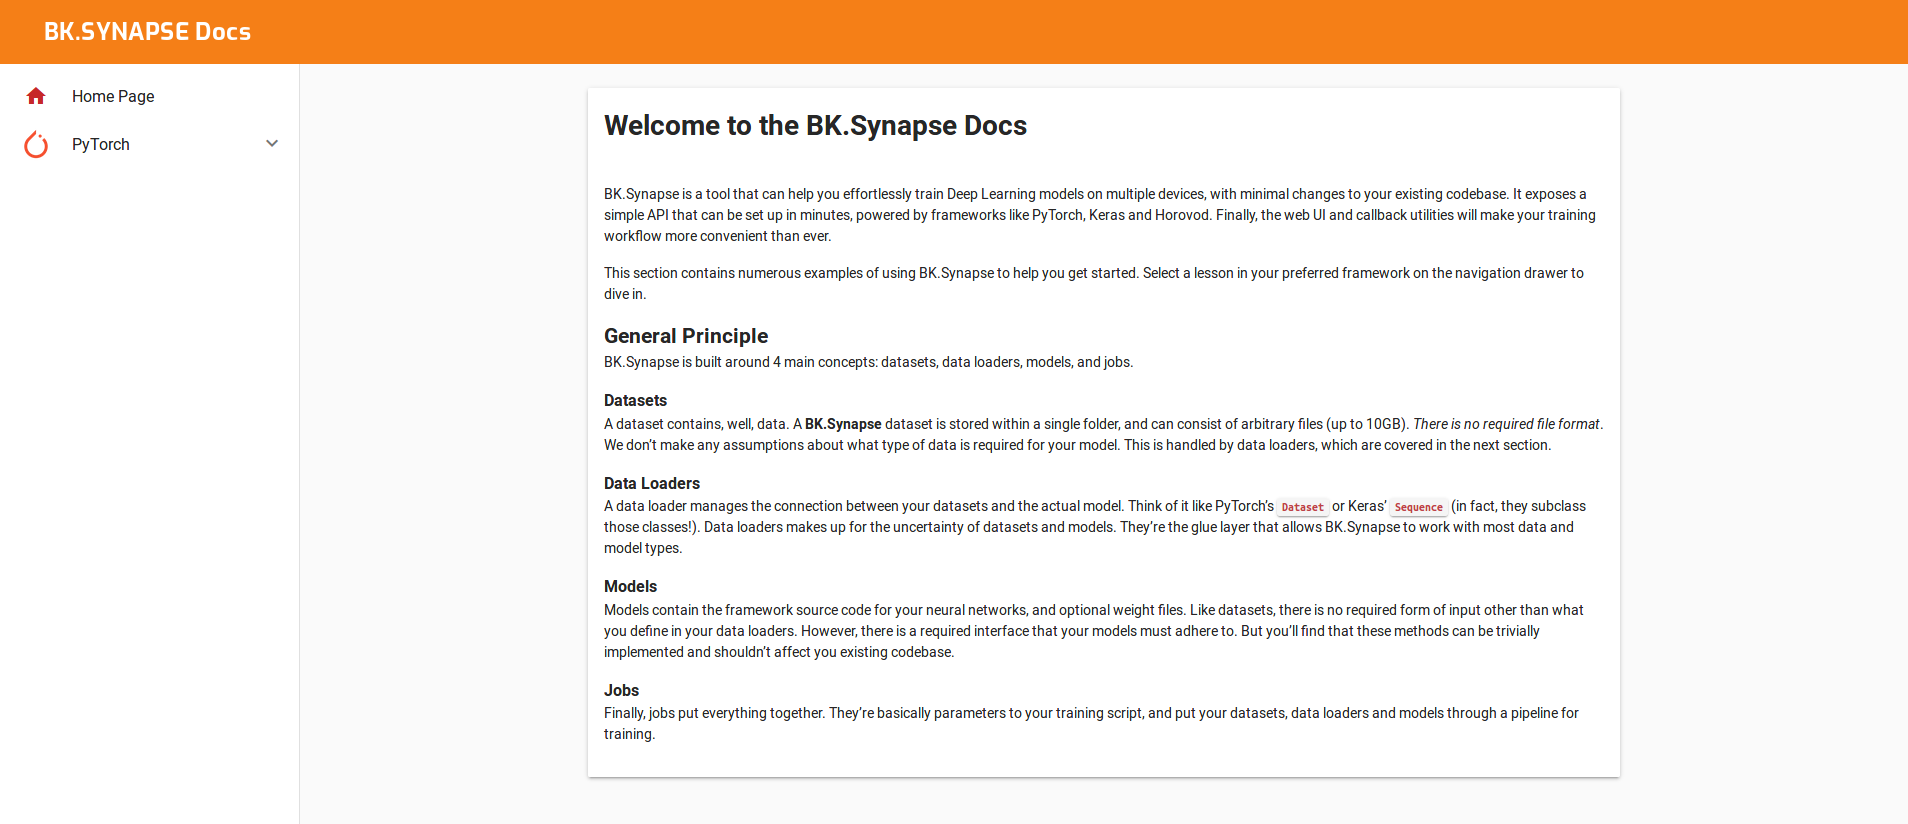
\includegraphics[width=0.95\textwidth,frame]{bks_example_7.png}
	\caption{Documentation and tutorials page}
	\label{fig:example-7}
\end{figure}

\chapter{Example model output}
Some examples of the trained model's output are shown the below figures. The predicted boxes are in red.

\begin{figure}[ht!]
    \centering
        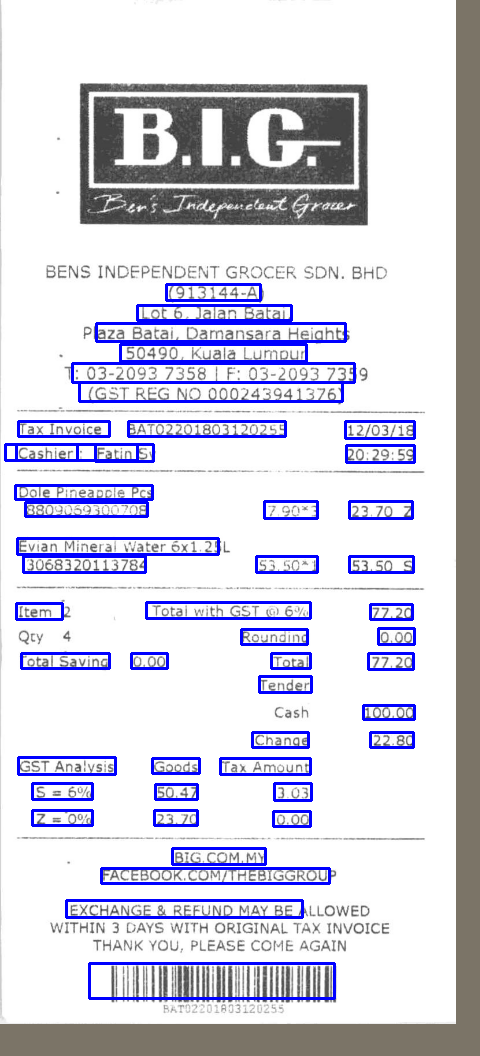
\includegraphics[height=0.47\textheight,frame]{rn-result-2.png}
    \caption{RetinaNet-101-DA output on the test set (1)}
	\label{fig:rn-results-2}
\end{figure}

\begin{figure}[ht!]
    \centering
        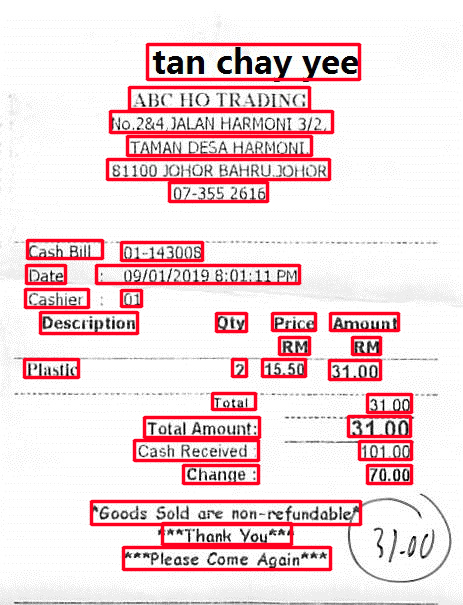
\includegraphics[width=0.7\textwidth,frame]{rn-result-1.png}
    \caption{RetinaNet-101-DA output on the test set (2)}
	\label{fig:rn-results-1}
\end{figure}

\begin{figure}[ht!]
    \centering
        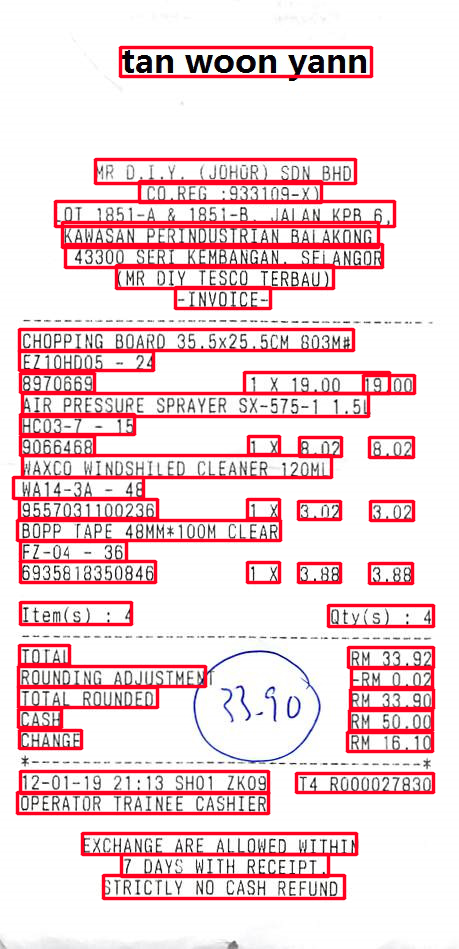
\includegraphics[width=0.7\textwidth,frame]{rn-result-3.png}
    \caption{RetinaNet-101-DA output on the test set (3)}
	\label{fig:rn-results-3}
\end{figure}

\begin{figure}[ht!]
    \centering
        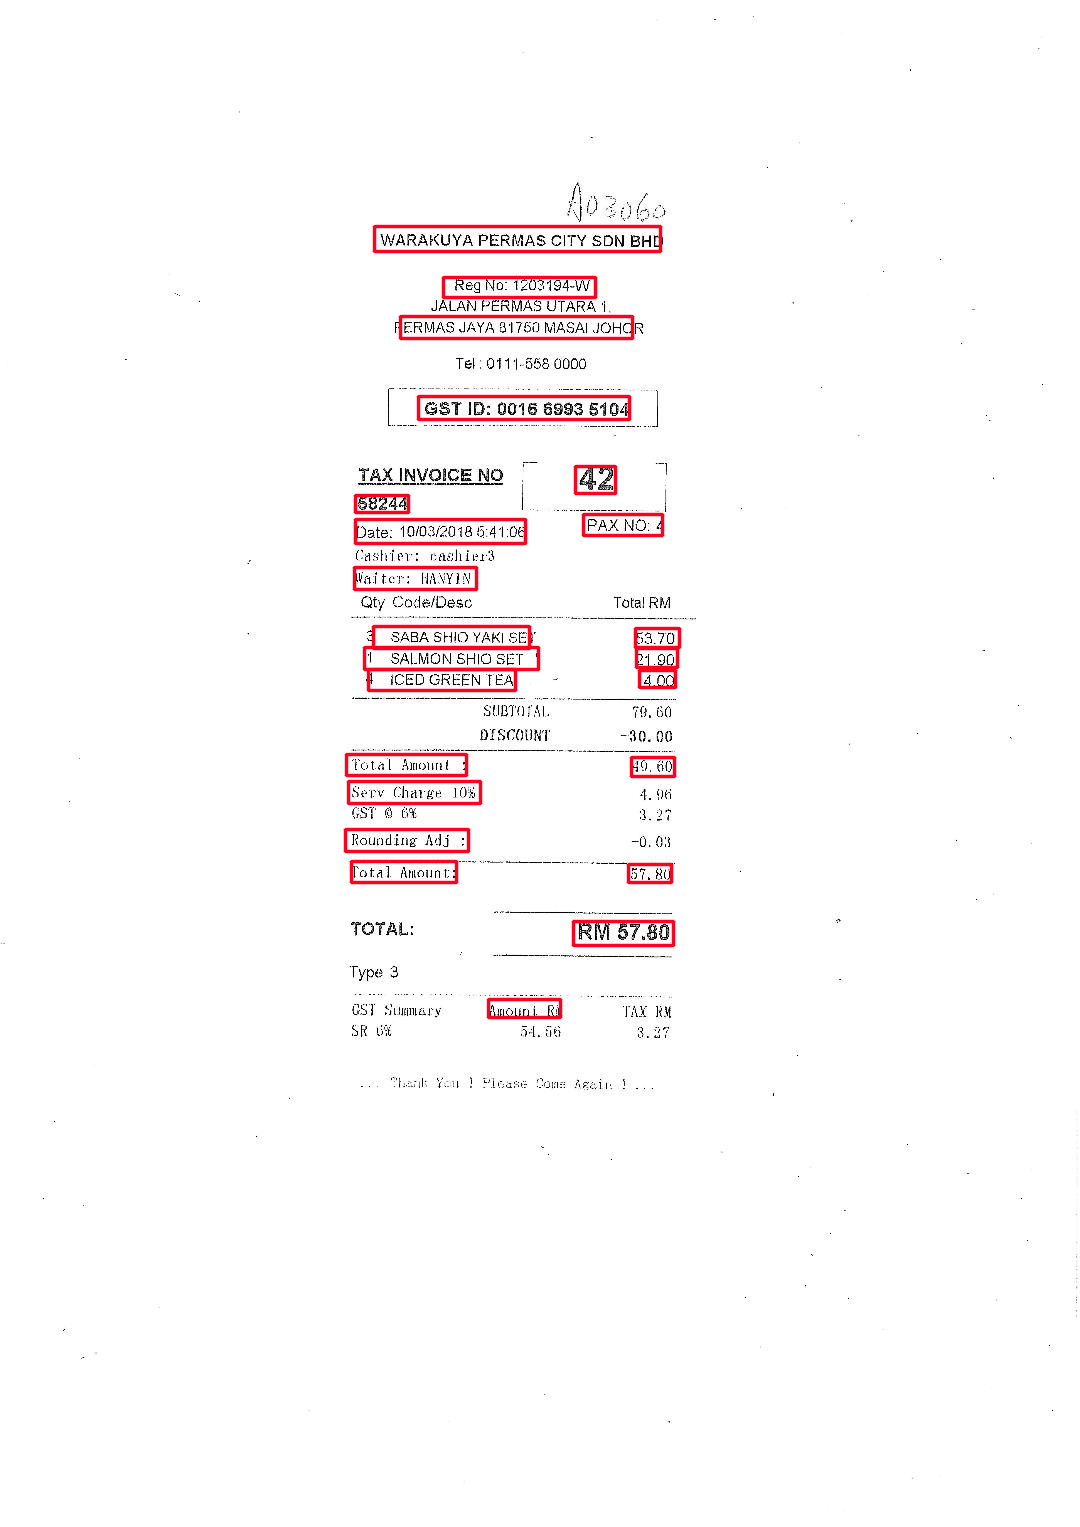
\includegraphics[width=0.7\textwidth,frame]{rn-result-4.png}
    \caption{RetinaNet-101-DA output on the test set (4)}
	\label{fig:rn-results-4}
\end{figure}
